%% Neuro-Symbolic Safe Highway Driving — Report
%% Compile: pdflatex report.tex  (run twice for cross-refs)
\documentclass[11pt,a4paper]{article}

\usepackage[margin=1in]{geometry}
\usepackage{graphicx}
\usepackage{booktabs}
\usepackage{amsmath,amssymb}
\usepackage{xcolor}
\usepackage{hyperref}
\usepackage{parskip}
\usepackage{microtype}
\usepackage{caption}
\usepackage{subcaption}
\usepackage{array}
\usepackage{enumitem}

\definecolor{urlblue}{RGB}{31,119,180}

\hypersetup{
  colorlinks=true,
  linkcolor=black,
  urlcolor=urlblue,
  citecolor=black
}

\captionsetup{font=small, labelfont=bf}

\title{\textbf{Neuro-Symbolic Reinforcement Learning\\for Safe Autonomous Highway Driving}\\[6pt]
\large LTL-Shielded Deep Q-Networks on HighwayEnv}
\author{Prateek Ganguli}
\date{April 2026}

\begin{document}
\maketitle

\noindent
Code: \url{https://github.com/pganguli/nsai-highway}

% ─────────────────────────────────────────────────────────────────────────────
\section{Application}

The agent controls an ego vehicle on a 4-lane highway populated with 50 surrounding vehicles using the HighwayEnv simulator~\cite{leurent2018}. At each time-step the agent receives a kinematic observation and selects one of five meta-actions: \textsc{lane\_left}, \textsc{idle}, \textsc{lane\_right}, \textsc{faster}, and \textsc{slower}. The objective is to maximize speed in the rightmost lane without colliding. The environment is stochastic: surrounding vehicles spawn at random positions each episode, travel at varying speeds, and occasionally merge across lanes.

The observation is a matrix \(\mathbf{o}_t \in \mathbb{R}^{10 \times 5}\), where each row represents one of the 10 nearest vehicles (including the ego). The five features per row are: presence (binary slot occupancy), longitudinal distance \(\Delta x\), lateral distance \(\Delta y\), relative longitudinal speed \(\Delta v_x\), and relative lateral speed \(\Delta v_y\), all in ego-relative coordinates normalized to \([-1, 1]\). Rows are sorted by longitudinal distance; vehicles behind the ego are included. The per-step reward is:
\[
  r_t = \frac{0.4\,r_\text{speed} + 0.1\,r_\text{lane} - \mathbf{1}_\text{crash} + 1}{1.5}
  \cdot \mathbf{1}_\text{on-road}
\]
where \(r_\text{speed} \in [0,1]\) increases linearly from 20 to 30\,m/s and \(r_\text{lane}\) rewards the rightmost lane. A crash or departure from the road terminates the episode.

% ─────────────────────────────────────────────────────────────────────────────
\section{Neuro-Symbolic Checklist}

\paragraph{1. The neural component.}
The neural component is a Double Deep Q-Network with a DeepSet backbone, trained via Prioritized Experience Replay for 100\,000 time-steps. It learns a Q-function \(Q_\theta(s, a)\) mapping states and actions to expected returns, discovering lane-change and speed-control strategies through reward feedback alone. It has no explicit knowledge of safety rules.

\paragraph{2. The symbolic component.}
The symbolic component is a Linear Temporal Logic (LTL) safety shield that evaluates four hard constraints at every time-step and removes any action that would violate them before the Q-network selects from the remaining candidates. No training is involved; the predicates are computed directly from the kinematic observation. Each blocked action is traceable to a named rule (\(\varphi_i\)).

\paragraph{3. Generalization of the neural component.}
Because vehicle row order shifts each time-step as relative distances change, a standard flat MLP is sensitive to this permutation. The DeepSet applies a shared encoder \(\phi\) to each vehicle independently and sums the resulting embeddings, making the representation permutation-invariant by construction. The continuous reward signal with respect to speed provides stable gradients across diverse traffic configurations.

\paragraph{4. Fragility of the symbolic component.}
The four predicates (\(\varphi_1\)--\(\varphi_4\)) cover the most common unsafe scenarios but leave gaps: diagonal cut-ins faster than the TTC threshold, simultaneous multi-vehicle threats, and spawn-overlap crashes (where a vehicle is initialized directly adjacent to the ego) fall outside the constrained set. The distance and TTC thresholds are fixed at 20\,m and 2.0\,s and may not transfer to different speed regimes or traffic densities without re-tuning.

\paragraph{5. Why the combination outperforms either component alone.}
After removing spawn-induced crashes, the pure neural and pure symbolic agents reach nearly identical crash rates (23.2\% vs 23.5\%). Hard rules alone add nothing beyond what reward-trained behavior achieves, and unconstrained reward optimization does not produce safe behavior either. The shielded agent reaches 18.0\%, a reduction attributable to the policy training within a constrained action set from the start: the Q-function never learns to value unsafe actions, so the shield's intervention rate falls as training progresses. Reward standard deviation also falls by 30\%, reflecting fewer high-penalty crash episodes.

% ─────────────────────────────────────────────────────────────────────────────
\section{Technique}

Three agents were compared: a pure neural agent, a pure symbolic finite-state machine (FSM), and a neuro-symbolic agent combining the neural architecture with the LTL shield. All three share the same HighwayEnv configuration and evaluation protocol. The neural and neuro-symbolic agents are built on Pearl~\cite{pearl2023}, Meta's modular reinforcement learning framework.

The neural agent uses a DeepSet Q-Network~\cite{zaheer2017}. The encoder \(\phi\) is a shared two-layer MLP \([5 \to 64 \to 64]\) applied independently to each of the 10 vehicle rows. The embeddings are summed element-wise to a 64-dimensional state representation, which is concatenated with a 5-dimensional one-hot action vector. The Q-value head \(\rho\), a two-layer MLP \([69 \to 256 \to 256 \to 1]\), outputs a scalar Q-value per (state, action) pair. Training uses Double Q-learning with a separate target network (updated every 50 steps) to reduce overestimation bias, and Prioritized Experience Replay (PER) with priority exponent \(\alpha = 0.6\) and importance-sampling exponent \(\beta\) annealed from \(0.4\) to \(1.0\). Key hyperparameters: learning rate \(5 \times 10^{-4}\), discount \(\gamma = 0.8\), replay buffer capacity 15\,000, batch size 32, and \(\varepsilon\)-greedy exploration from \(1.0\) to \(0.05\) over the first 10\,000 steps.

The LTL shield enforces four globally-valid (\(G\)) constraints at every time-step:
\begin{align*}
  \varphi_1 &: G\bigl(d_\text{front} > 20\,\text{m}\bigr) & &\text{no tailgating}\\
  \varphi_2 &: G\bigl(\tau_\text{front} > 2.0\,\text{s}\bigr) & &\text{minimum time-to-collision}\\
  \varphi_3 &: G\bigl(\textsc{LaneLeft} \Rightarrow \neg\, o_\text{left}\bigr) & &\text{left lane clear before merging}\\
  \varphi_4 &: G\bigl(\textsc{LaneRight} \Rightarrow \neg\, o_\text{right}\bigr) & &\text{right lane clear before merging}
\end{align*}
A critical design choice is that the shield is integrated as action masking inside the environment wrapper (\texttt{ShieldedHighwayPearlEnv}), not applied as a post-hoc override after the agent commits to an action. After each step, the wrapper computes the safe action subset for the resulting next state \(s'\) and stores it in the replay buffer. The Bellman backup therefore uses:
\[
  y = r + \gamma \max_{a' \in \mathcal{A}_\text{safe}(s')} Q_{\bar\theta}(s', a')
\]
Without this, the replay buffer records the proposed (unsafe) action while the environment executes a different (safe) one, creating an off-policy error that corrupts Q-value estimates. The shield is also exposed as a Pearl \texttt{SafetyModule} (class \texttt{LTLShieldSafetyModule}), making it composable with other Pearl components. A small penalty (\(-0.05 \times n_\text{blocked}/5\) per step) is subtracted from the reward whenever the shield filters actions, encouraging the policy to reach the same safe action that the shield would approve.

The symbolic FSM requires no training. It has four states (CRUISE, FOLLOW, OVERTAKE\_L, KEEP\_RIGHT) and applies a fixed decision tree over kinematic predicates with thresholds 20\% tighter than the LTL shield. It provides a lower bound on the reward achievable by static rule-based control and an upper bound on the safety that fixed rules can guarantee in this environment.

% ─────────────────────────────────────────────────────────────────────────────
\section{Results}

\subsection{Evaluation Setup and Metrics}

All three agents were evaluated under identical conditions: 100 independent episodes per agent, greedy policy, and identical random seeds. The environment uses 4 lanes, 50 surrounding vehicles, a 60-second episode limit, and \texttt{offroad\_terminal = True}. The neural and neuro-symbolic agents each used the checkpoint with the highest evaluation reward on 5 greedy episodes during training; no checkpoint is shared between them. The FSM uses no checkpoint.

Four metrics were collected per episode: cumulative reward (primary performance measure), mean speed in m/s, a binary crash indicator, and episode length in steps. Crash rate is the fraction of episodes ending in a collision. A supplementary filtered analysis removes episodes that crashed within the first 5 steps, since HighwayEnv occasionally places the ego vehicle in an immediately un-drivable initial configuration. These early crashes reflect environment initialization variance rather than policy behavior, so filtering isolates planner-attributable crashes.

\subsection{Evaluation}

\begin{table}[h]
  \centering
  \caption{Evaluation results over all 100 episodes.}
  \label{tab:all}
  \resizebox{\linewidth}{!}{%
    \begin{tabular}{lrrrr}
      \toprule
      Agent & Reward (\(\uparrow\)) & Reward Std (\(\downarrow\)) & Speed m/s (\(\uparrow\)) & Crash Rate (\(\downarrow\)) \\
      \midrule
      Pure Neural (Pearl DQN)            & \textbf{45.73} & 16.32          & \textbf{27.39} & 27\% \\
      Pure Symbolic (FSM)                & 38.30          & 14.83          & 22.95          & 25\% \\
      Neuro-Symbolic (Shielded DQN)      & 40.80          & \textbf{11.44} & 23.03          & \textbf{18\%} \\
      \bottomrule
  \end{tabular}}
\end{table}

\begin{table}[h]
  \centering
  \caption{Evaluation with spawn-induced crashes removed (episodes crashing within 5 steps excluded).}
  \label{tab:filtered}
  \resizebox{\linewidth}{!}{%
    \begin{tabular}{lrrrrr}
      \toprule
      Agent & \(n\) & Reward (\(\uparrow\)) & Reward Std (\(\downarrow\)) & Speed m/s (\(\uparrow\)) & Crash Rate (\(\downarrow\)) \\
      \midrule
      Pure Neural (Pearl DQN)            & 95  & \textbf{48.02} & 13.26          & \textbf{27.53} & 23.2\% \\
      Pure Symbolic (FSM)                & 98  & 39.00          & 14.13          & 22.92          & 23.5\% \\
      Neuro-Symbolic (Shielded DQN)      & 100 & 40.80          & \textbf{11.44} & 23.03          & \textbf{18.0\%} \\
      \bottomrule
  \end{tabular}}
\end{table}

\begin{figure}[htbp]
  \centering
  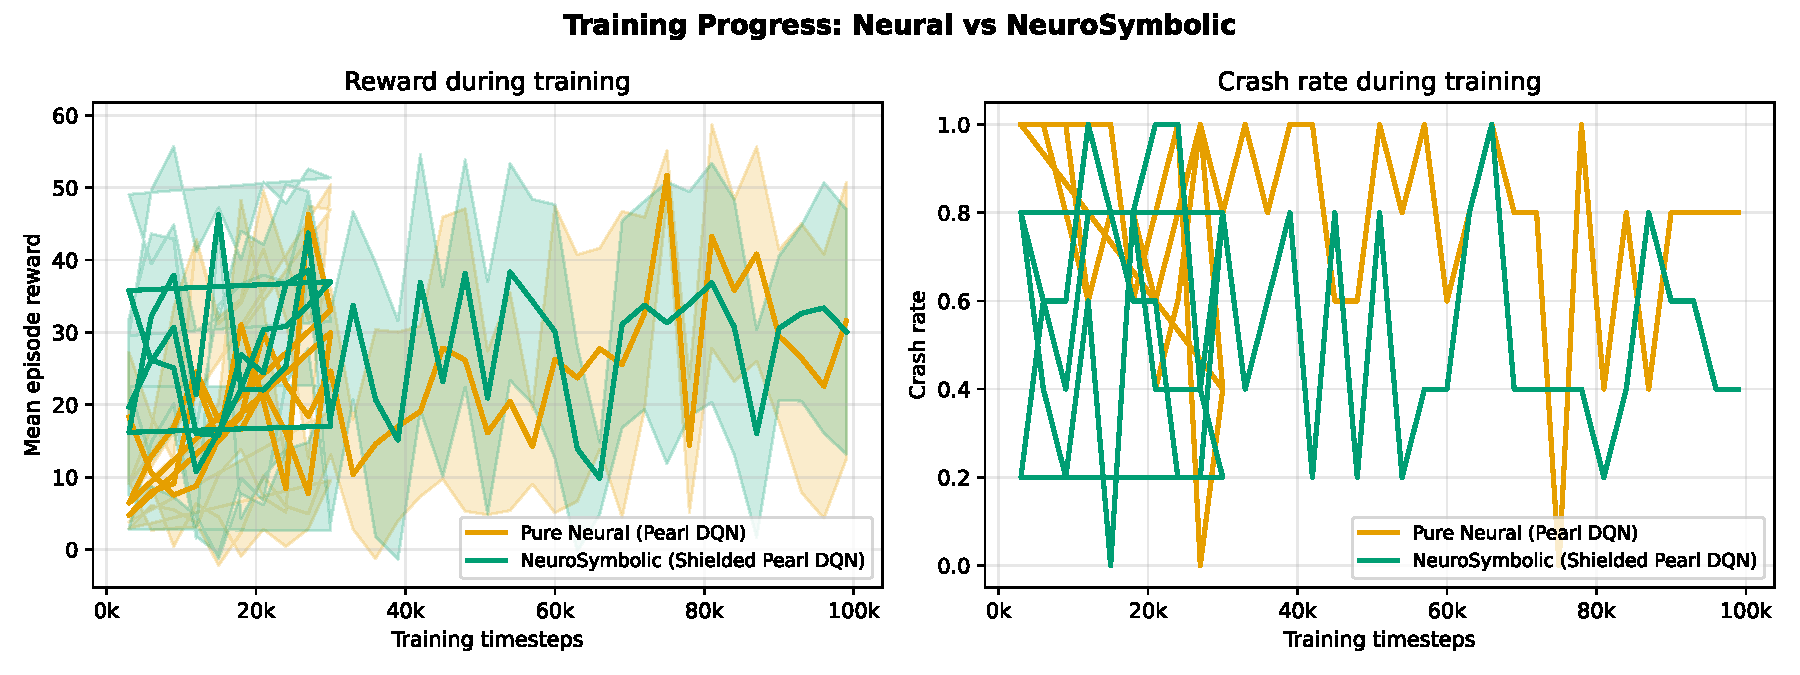
\includegraphics[width=\linewidth]{fig1_training_curves.pdf}
  \caption{Training reward and crash rate vs.\ time-step (100k steps) for the neural and neuro-symbolic agents.}
  \label{fig:training}
\end{figure}

\begin{figure}[htbp]
  \centering
  \begin{subfigure}{\linewidth}
    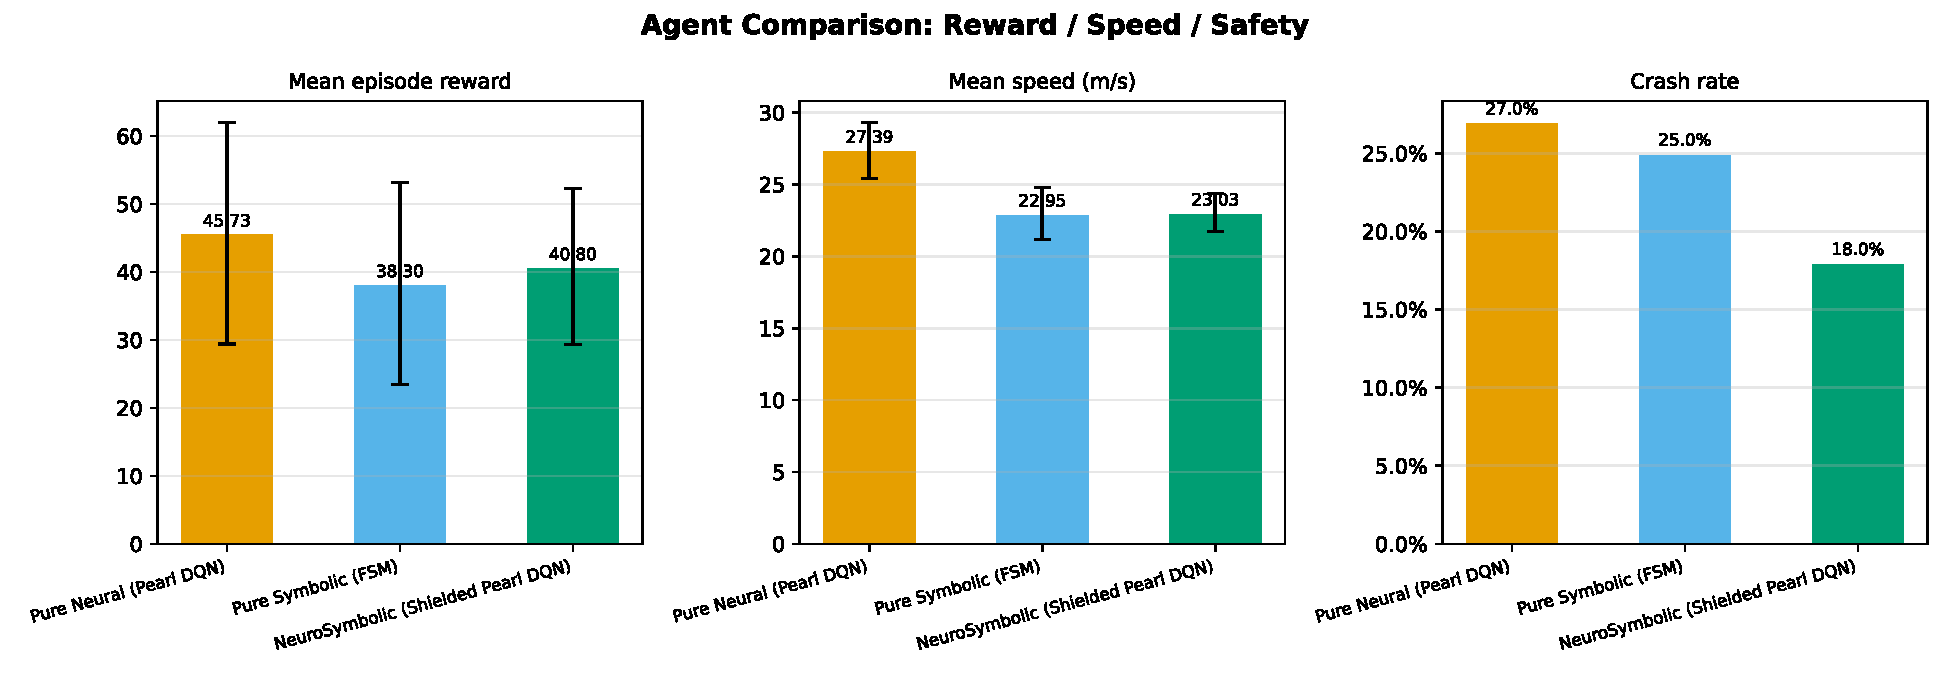
\includegraphics[width=\linewidth]{fig2_bar_comparison.pdf}
    \caption{All 100 episodes.}
  \end{subfigure}
  \begin{subfigure}{\linewidth}
    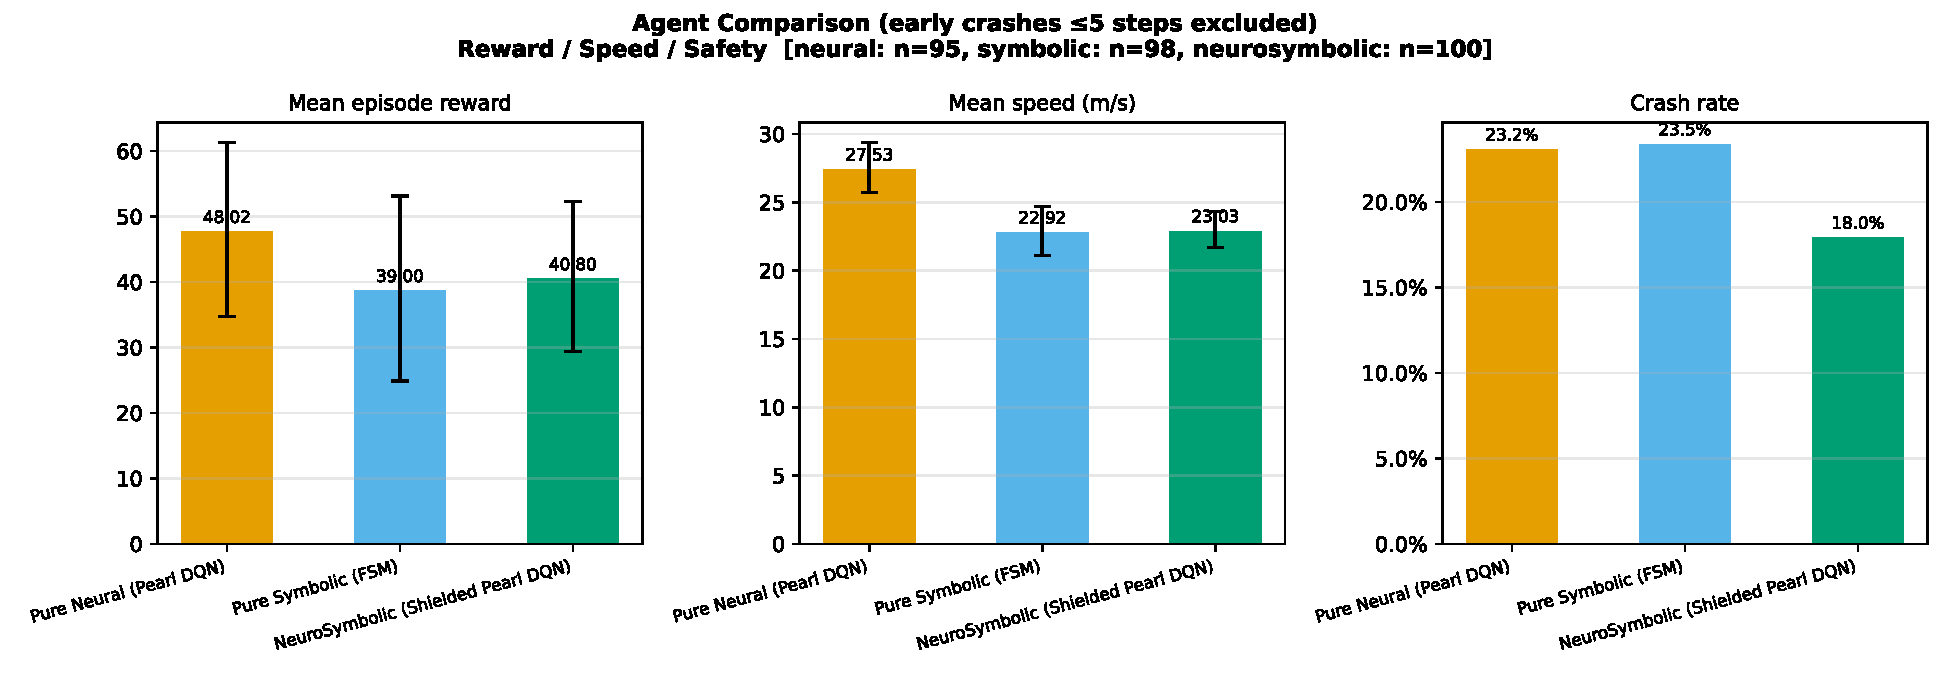
\includegraphics[width=\linewidth]{fig5_bar_comparison_filtered.pdf}
    \caption{Spawn-induced crashes removed.}
  \end{subfigure}
  \caption{Bar comparison across all three agents on reward, speed, and crash rate.}
  \label{fig:bars}
\end{figure}

\begin{figure}[htbp]
  \centering
  \begin{subfigure}{\linewidth}
    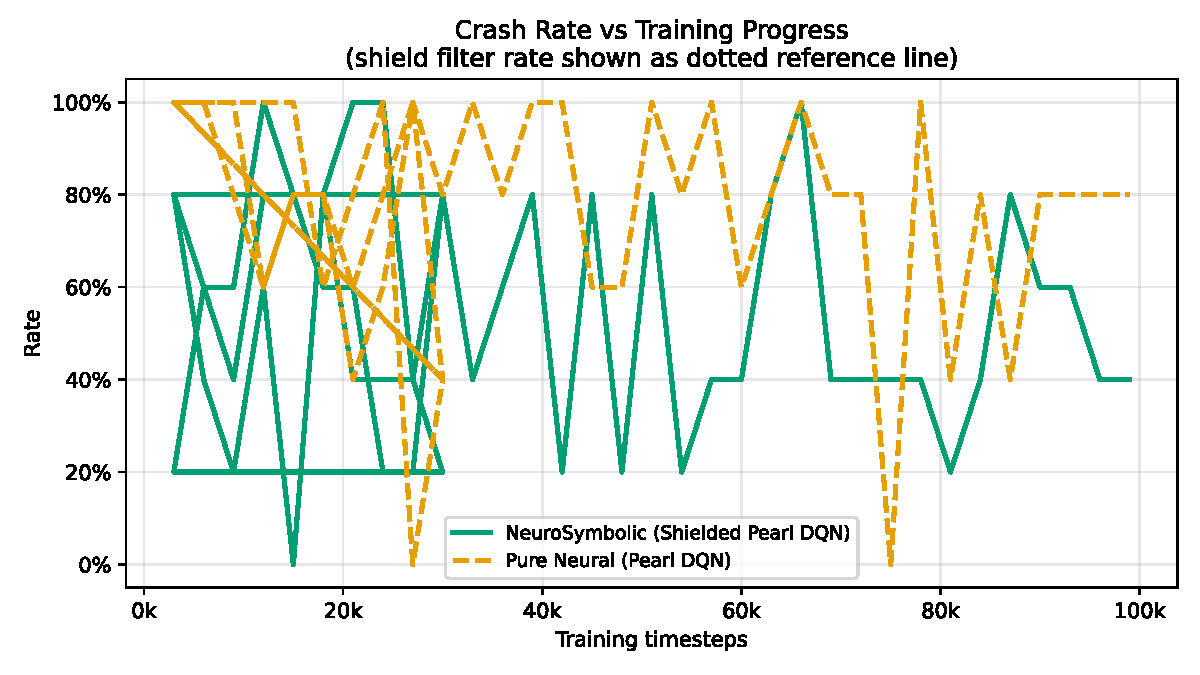
\includegraphics[width=\linewidth]{fig3_shield_filter.pdf}
    \caption{Shield override rate during training.}
  \end{subfigure}
  \begin{subfigure}{\linewidth}
    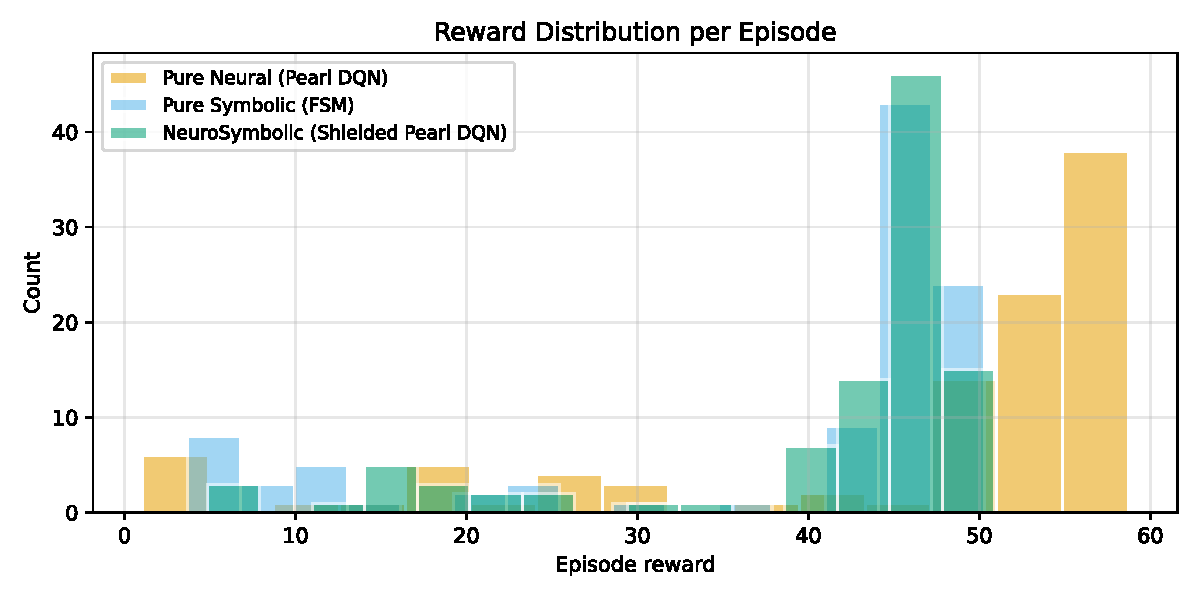
\includegraphics[width=\linewidth]{fig4_reward_distribution.pdf}
    \caption{Per-episode reward distributions (100 episodes).}
  \end{subfigure}
  \caption{Training dynamics and reward spread across agents.}
  \label{fig:diag}
\end{figure}

\subsection{Discussion}

The neuro-symbolic agent achieves the lowest crash rate (18\%) and the lowest reward standard deviation (11.44). It gives up roughly 5 reward points versus the unconstrained neural agent (40.80 vs 45.73) while eliminating 9 percentage points of crash rate. After removing spawn-induced crashes, the neural and symbolic agents' crash rates converge to 23.2\% and 23.5\% respectively, confirming that the FSM's apparent safety advantage in the full dataset comes entirely from 2 fewer spawn crashes it encountered by chance rather than from its conservative thresholds. The 5.2-percentage-point gap between the shielded agent and both baselines holds after filtering, identifying it as a planner-attributable reduction. The declining shield override rate in Figure~\ref{fig:diag} (left) shows the policy learning to select actions that the shield approves without intervention.

The FSM is the weakest agent on both axes: it achieves lower reward than unconstrained neural training (38.30 vs 45.73) while offering no safety advantage once the evaluation is controlled for spawn effects. Hard-coded rules with fixed thresholds cannot adapt to the full diversity of traffic configurations that arise over 100 evaluation episodes. The neuro-symbolic result demonstrates that safety constraints and reward maximization are compatible when the shield is applied at the environment level as action masking: the Q-function is shaped from the start to operate within safe limits, rather than being corrected by a post-hoc override that would corrupt its value estimates.

% ─────────────────────────────────────────────────────────────────────────────
\begin{thebibliography}{9}

  \bibitem{leurent2018}
  Leurent, E. (2018). An Environment for Autonomous Driving Decision-Making.
  \textit{GitHub}. \url{https://github.com/eleurent/highway-env}

  \bibitem{zaheer2017}
  Zaheer, M., Kottur, S., Ravanbakhsh, S., P\'{o}czos, B., Salakhutdinov, R., and Smola, A. (2017).
  Deep Sets. \textit{Advances in Neural Information Processing Systems (NeurIPS)}, 30.

  \bibitem{alshiekh2018}
  Alshiekh, M., Bloem, R., Ehlers, R., K\"{o}nighofer, B., Niekum, S., and Topcu, U. (2018).
  Safe Reinforcement Learning via Shielding.
  \textit{Proceedings of the AAAI Conference on Artificial Intelligence}, 32(1).

  \bibitem{pearl2023}
  Zhu, Z., Dong, H., et al. (2023). Pearl: A Production-Ready Reinforcement Learning Agent.
  Meta Research. \url{https://github.com/facebookresearch/Pearl}

\end{thebibliography}

\end{document}
